% cjupiter-c3-2.tex

\documentclass{standalone}
% jupiter-illustration-preamble.tex

\usepackage{tikz}
\usetikzlibrary{shapes, positioning, arrows.meta, calc, backgrounds, fit}

\def\hdist{1.8}
\def\vdist{2.0}
\tikzset{node distance = \vdist and \hdist}

\tikzset{every lower node part/.style = {red}}
\newcommand{\statesplit}[4]{% #1: state upper label; #2: state lower label; #3: position; #4: name
  \node (#4) [circle split, draw, minimum size = 6mm, text width = 10mm, align = center, #3, font = \Large]
  {
    $#1$
    \nodepart{lower}
    $#2$
  };
}

\newcommand{\rectsplit}[2]{% #1: state upper label; #2: state lower label
  \node [draw, rectangle split, rectangle split parts = 2, 
    align = center, font = \Large]
  {
    #1
    \nodepart{two}
    \textcolor{red}{#2}
  };
}

\newcommand{\transition}[4][]{% #2: start state; #3: end state; #4: transition label; #1: transition label position (optional)
  \draw[>=Stealth, ->] (#2) to node (#2to#3) [rectangle, draw, above = 2pt, sloped, #1, font = \small] {$#4$} (#3);
}

\newcommand{\set}[1]{\{#1\}}
\newcommand{\ins}[2]{\textsc{Ins}(#1,#2)}
\newcommand{\del}[2]{\textsc{Del}(#2)}
% \newcommand{\del}[2]{\textsc{Del}(#1,#2)}


\begin{document}
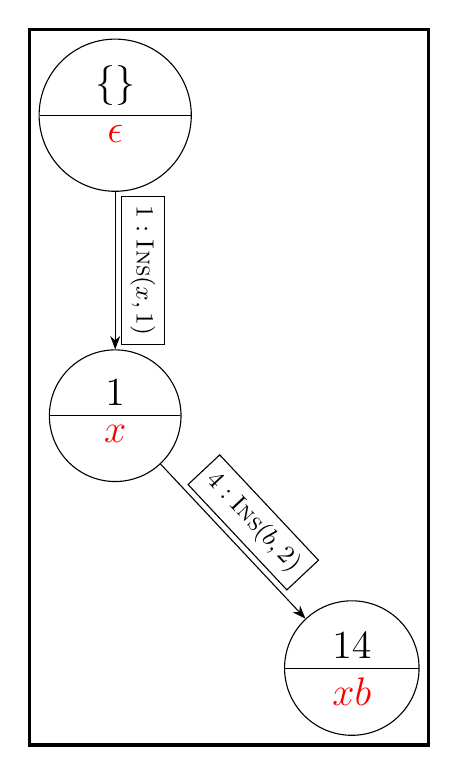
\begin{tikzpicture}[bg/.style = {rectangle, draw, very thick}]
  \statesplit{\{\}}{\epsilon}{}{0}

  \statesplit{1}{x}{below = of 0}{1}
  \transition{0}{1}{1: \ins{x}{1}}

  \statesplit{14}{xb}{below right = of 1}{14}
  \transition{1}{14}{4: \ins{b}{2}}

  \node () [fit = (0) (1) (14), bg] {};
\end{tikzpicture}
\end{document}
